\documentclass[acmsmall,nonacm,screen,review]{acmart}
\newif\ifEnableExtend
%\EnableExtendtrue
\EnableExtendfalse

\usepackage[utf8]{inputenc}
\usepackage{url}
\usepackage{color}
\newcommand{\csch}[1]{{\color{red} Christian says: #1}}
\newcommand{\Is}       {:=}
\newcommand{\set}[1]{\left\{ #1\right\}}
\newcommand{\sodass}{\,:\,}
\newcommand{\setGilt}[2]{\left\{ #1\sodass #2\right\}}
\usepackage{amsmath}
\usepackage{amsthm}
\usepackage{xspace}
\usepackage{relsize}

\usepackage{multirow}
\usepackage{wrapfig}

\newtheorem{openproblem}{Open Problem}
\newcommand{\ie}{i.\,e.,\xspace}
\newcommand{\eg}{e.\,g.,\xspace}
\newcommand{\etal}{et~al.\xspace}
\newcommand{\cov}{\term{cov}\xspace}
\newcommand{\term}[1]{\textsl{#1}}
\newcommand{\Comment}[1]{\textsl{#1}}
\DeclareMathOperator{\vol}{vol}
\DeclareMathOperator{\origVol}{origVol}
\DeclareMathOperator{\origDeg}{origDeg}
\DeclareMathOperator{\numPins}{numPins}
%%%%%%%%%%%%%%%%%%%%%%%%%%%%%
\setcopyright{none}
\copyrightyear{2024}
\acmYear{2021}
\acmDOI{}
\acmPrice{}
\acmISBN{}

\title{Beginner's Practical: \\ Hypergraph Conductance-based Clustering}
\author{Mariia Meshchaninova}
\email{mariia.meshchaninova@stud.uni-heidelberg.de, Informatik B.Sc. 100\%, 4740180}
\affiliation{%
  \institution{Heidelberg University}
  \streetaddress{Im Neuenheimer Feld 205}
  \city{Heidelberg}
  \state{Baden-Württemberg}
  \country{Germany}
  \postcode{69120}
}


\date{}

\begin{document}

\begin{abstract}
%Insert abstract here.
Hypergraph clustering is a problem of partitioning the nodes of a 
hypergraph into "true clusters" which are densely connected internally 
and sparsely connected externally. Conductance is a metric measuring 
the quality of a cut which is defined as the ratio of the weight of 
the cut to the minimal volume of one side of the cut.

In this project, we implement a hypergraph clustering algorithm that
heuristically tries to minimize the maximum value of the conductance 
over all cuts between clusters to find a high-quality hypergraph 
clustering. The algorithm is based on the existing shared-memory 
parallel algorithm for hypergraph partitioning \texttt{Mt-KaHyPar}.

Experimental results show that our implementation is able to find
high-quality conductance-wise hypergraph clustering in a short time,
but the results are heavily dependent on the parameter $k$ of the 
estimated number of clusters.
\end{abstract}
\maketitle

\section{Introduction}
Hypergraph clustering is a problem of partitioning the nodes of a 
hypergraph into "true clusters" which are densely connected internally 
and sparsely connected externally. It is useful in many applications, 
such as semi-supervised learning \cite{ApplicationLearning}, 
gene expression analysis \cite{ApplicationGeneExpression}
and image segmentation \cite{ApplicationImageSegmentation}. 
Conductance metric, which is defined for a cut as the ratio of the cut 
weight to the minimal volume of one side of the cut, is widely used in 
graph clustering \cite{PCde, GraphConductance2006} but to the best
of our knowledge, there are no partitioners directly optimizing
conductance-based metric of a hypergraph. However, conductnace has been 
applied as a metric for evaluating the quality of a hypergraph 
clustering \cite{HyperSF}. Therefore in this project, we implement a 
heuristic hypergraph clustering algorithm with the objective of 
minimizing the maximum value of the conductance over all cuts between 
the clusters while partitioning the hypargraph in at most $k$ clusters. 

\noindent Our algorithm is based on the existing shared-memory parallel 
hypergraph $k$-way partitioner \texttt{Mt-KaHyPar} and uses the same 
multilevel approach as the original algorithm. First, the hypergraph is 
coarsened in stages by detecting and merging local node clusters, then 
the coarsest hypergraph is partitioned into $k$ clusters, and finally 
the initial partitioning is refined by uncoarsening the hypergraph 
nodes and applying a local search algorithm to improve the given 
objective. We implement two objective functions for the local search 
algorithm - \textit{conductance\_local} and 
\textit{conductance\_global} - and compare their performance on the
circuit-based benchmark set \textit{ISPD98} \cite{IBMBenchmark} against 
a state of the art hypergraph clustering algorithm 
\texttt{HyperModularity}. We also conduct a scaling experiment to 
evaluate the performance of our algorithm one multiple cores.

\noindent In following, we define the used concepts in 
Section~\ref{sec:preliminaries}, then we shortly describe related work 
on hypergraph and conductance-based clustering in 
Section~\ref{sec:related_work}. In Section~\ref{sec:implementation}, 
we describe the implementation of the new objectives for optimizing 
the conductance and their integration in \texttt{Mt-KaHyPar}. 
Afterwards, we present the experimental results of our implementation 
in Section~\ref{sec:experiments}. Finally, we conclude the report 
with a shoret summary of the results in Section~\ref{sec:conclusion}.


%\noindent In this project, we implement a heuristic algorithm for hypergraph 
%lustering with the aim of partitioning the nodes of a hypergraph into 
%at most $k$ clusters, while minimising the maximum value of the conductance 
%over all the cuts between the clusters. The algorithm is based on the 
%existing shared-memory parallel hypergraph partitioner \texttt{Mt-KaHyPar}
%and uses the same multilevel approach as the original algorithm. First,
%the hypergraph is coarsened in stages by detecting and merging node
%commubities, then the coarsest hypergraph is partitioned into $k$ clusters, 
%and finally the initial partitioning is refined by uncoarsening the 
%hypergraph nodes and applying a local search algorithm to improve the given 
%objective. We implement two objective functions for the local search 
%algorithm - \textit{conductance\_local} and \textit{conductance\_global} - 
%ans compare their performance on a benchmark set of instances against



%performance on large benchmark sets of instances against other state-of-the-art 
%hypergraph partitioners \cite{MtKaHyPar2020}. The algorithm follows a multilevel
%approach by in stages coarsening a given hypergraph via detecting and merging 
%communities of the nodes, then partitioning the coarsest hypergraph into $k$ 
%clusters, and then iteratively refining the initial partitioning by uncoarsening
%the hypergraph nodes and applying a local search algorithm to improve the given 
%objective. The original algorithms supports several objectives, such as minimizing 
%the weight of the cut (\textit{cut} metric) or the sum of the external degrees of 
%the clusters (\textit{soed} metric). In this project, we implement two additional 
%objective functions for the \texttt{Mt-KaHyPar} algorithm to minimize the overall 
%maxmal conductance of a cut inbetween the clusters: \textit{conductance\_local} 
%and \textit{conductance\_global}.


\section{Preliminaries}
\label{sec:preliminaries}

In this section, we give an overview of the used concepts and 
notations and at the end define conductance of a hypergraph.

\smallbreak
\noindent\textbf{Hypergraph} is a generalization of a graph, where a 
hyperedge connects one, two or more nodes. Formally, an edge-weighted 
hypergraph $H = (V, E, \omega)$ consists of a non-empty set of nodes 
$V$, a set of hyperedges (also called \textit{nets} or simply 
\textit{edges}) $E \subseteq 2^V$ and a weight function for 
hyperedges $\omega: E \to \mathbb{N}$. In case of unweighted 
hyperedges, we set $\omega(e) = 1$ for all $e \in E$. 

\smallbreak
\noindent\textbf{$k$-way clustering} of a hypergraph 
$H = (V, E,\omega)$ is a partitioning of the set of nodes $V$ into 
$k$ disjoint subsets $V_1, \dots, V_k$ called \textit{clusters}. Empty 
clusters are allowed, so $k$ is only an upper bound on the final 
number of clusters. Our algorithm is allowed to eventially move all 
the nodes of a cluster to other clusters if it would be beneficial 
for the objective function. 

\smallbreak
\noindent\textbf{Cut} $\partial S$ of a hypergraph 
$H = (V, E, \omega)$ is partitioning of the set of nodes $V$ into 
two disjoint non-empty subsets $S$ and $V \backslash S$. A hyperedge 
$e \in E$ is called a \textbf{cutting edge} of the cut $\partial S$ 
if it has at least one pin in $S$ and at least one pin in 
$V \backslash S$. The weight of the cut is defined as the sum of the 
weights of the cutting edges of the cut $\partial S$: 
\[\omega(\partial S) = \sum_{e \in \partial S} \omega(e)\]
Therefore in case of unweighted hyperedges, the weight of the cut is 
equal to the number of cutting edges of the cut.

\smallbreak
\noindent\textbf{Pin} of a hyperedge $e \in E$ is a node $v \in V$ 
such that $v \in e$. A hyperedge with only one pin is called a 
\textbf{sinle-pin net}. In the implementation, we use number of pins 
$\numPins_i(e)$ of a hyperedge $e \in E$ in a cluster $V_i$ to decide 
whether to move a node $v$ from one cluster $V_i$ to another cluster 
$V_j$.

\smallbreak
\noindent\textbf{Weighted degree} of a node $v \in V$ is defined the 
same way in hypergraphs as in graphs. It is the sum of the weights of 
all hyperedges $e \in E$ that contain the node $v$: 
\[\deg_\omega(v) = \sum_{e\in E: v \in E} \omega(e)\]
As during the coarsening phase of the algorithm we merge nodes, we 
also use \textbf{original weighted degree} of a node $v' \in V'$ 
of the coarsened hypergraph $\origDeg_\omega(v')$ which is defined as 
the sum of the weighted degrees of all nodes of the initial hypergraph 
$v \in V$ that were merged into $v'$ during the coarsening phase of 
the algorithm.

\smallbreak
\noindent\textbf{Volume} of a hypergraph $H = (V, E, c, \omega)$ is 
defined as the sum of the weighted degrees of all nodes $v \in V$. 
Analogously, we define the \textbf{volume of a cluster} $V_i$ as the 
sum of the weighted degrees of all nodes $v \in V_i$:
\[\vol(H) = \sum_{v \in V} \deg_\omega(v) \ \ \ \ \ \ \
\vol(V_i) = \sum_{v \in V_i} \deg_\omega(v)\]
And for the same reason as for the original weighted degree, we also 
define the \textbf{original volume} of a hypargraph and a cluster:
\[\origVol(H) = \sum_{v \in V} \origDeg_\omega(v) \ \ \ \ \ \ \
\origVol(V_i) = \sum_{v \in V_i} \origDeg_\omega(v)\]
This way, the original volume of a cluster or of the whole hypergraph 
in the coarsened hypergraph is equal to the corresponding volume in 
the initial - \textit{original} - hypergraph.

\smallbreak
\noindent\textbf{Conductance of a cut} $\partial S$ of a hypergraph 
$H = (V, E, \omega)$ is defined as the ratio of the weight of the cut 
to the minimum volume of one side of the cut. The maximal conductance 
of a cut In a hypergraph is referred to as the 
\textbf{conductance of the hypergraph}: 
\[{\varphi(S)} = \frac{\omega(\partial S)}{\min\{vol(S), vol(V \backslash S)\}}
\ \ \ \ \ \ 
{\varphi(V)} = \max_{\emptyset \subsetneq S \subsetneq V} \varphi(S)
\]
To use conductance as a quality metric for a hypergraph clustering 
with possibly more than two clusters, we define the 
\textbf{conductance of a hypergraph clustering} $V_1, \dots, V_k$ as 
the maximum conductance of all cuts between the clusters. 
Conveniently, this definition can be simplified to the maximal 
conductance of a cut $\partial V_i$ over all clusters $V_i$:
\[\varphi(V_1, \dots, V_k) 
:= \max_{I \subsetneq \{1, \dots, k\}:
                            \cup_{i \in I} V_i \neq \emptyset, V}
        \varphi(\cup_{i \in I} V_i) 
 = \max_{i = 1 \dots k: V_i \neq \emptyset, V} \varphi(V_i)\]
A proof of this nice statement can be found in Appendix~\ref{appendix:a}.

\section{Related Work}
\label{sec:related_work}

For graph clustering, there are several state of the art algorithms 
that aim to minimize the resulting conductance. Some of them are 
heuristic like the diffusion based \texttt{NIBBLE} \cite{Nibble} and 
\texttt{hk-relax} \cite{HKRelax}. Other, such as degree ratio-based 
\texttt{PC\_de} \cite{PCde} have a theoretical guaranatee of the 
resulting conductance. 

As for the hypergraph-clustering, to the best of our knowledge, there 
are no existing algorithms that directly optimize a conductance-based 
objective. Instead, state of the art hypergraph clustering algorithms, 
\eg \texttt{HyperModularity} which we use for comparison with our 
algorithm, deliver high quality hypergraph clustering by optimizing 
the modularity of the hypergraph 
\cite{HyperModularity,ModularityComparison}.

The algorithm \texttt{Mt-KaHyPar} that we use as a base for our 
implementation also optimizes the modularity of the hypergraph in its 
coarsening stage. But as whole, it could be seen as a framework 
for hypergraph partitioning with a user-implemented objective, which 
is optimized during the initial partitioning of the coarsest 
hypergraph and later in the uncoarsening stage consisting of label 
propagation and FR-refinement x\cite{MtKaHyPar2020}.

\section{Implementation}
\label{sec:implementation}

To implement our algorithm, we introduced a new objective function
for the \texttt{Mt-KaHyPar} algorithm, which provides a framework 
for hypergraph partitioning. Also, we introduced a clustering mode
(calles \texttt{cluster}) for the \texttt{Mt-KaHyPar} algorithm, which
relaxes weight constarints for the clusters. The idea and most of the
implementation of this mode was taken with a premission from
a fork of \texttt{Mt-KaHyPar} by Adil Chhabara: 
\hyperlink{https://github.com/adilchhabra/mt-kahypar}
{https://github.com/adilchhabra/mt-kahypar} 

\smallbreak
\noindent For a new objective function for \texttt{Mt-KaHyPar}, we 
needed to implement efficient calculation of the conductance of the 
clustering, formulate an initial partitioning algorithm to apply to 
the coarsest hypergraph and a define a gain function for the local 
search algorithm. In this section, we describe our approaches to
these tasks.

\subsection{Efficient Conductance Calculation}
\noindent\textbf{Conductance calculation} is needed to evaluate the
quality of the clustering and to stop the local search algorithm
when no more moves are worsening the conductance of the clustering.

Firstly, to be able to efficiently calculate the conductance of a clustering, 
we keep all original weighted degrees, original volumes and cut weights
up to date. This is done by adjusting their values during the changes of
the clustering or (un)coarsening of the hypergraph. Here are both these 
changes:

\begin{itemize}
    \item \textbf{(Un)contraction} of a group of nodes $v_1 \dots v_c$ into (from) 
one node $v'$:
\begin{itemize}
    \item $\origDeg_\omega(v') = \origDeg_\omega(v_1) + \dots + \origDeg_\omega(v_c)$. 
Hence, atomical substraction (addition) is enough to update the original 
weighted degrees; It is important to note that this operation doesn't increase 
the run-time complexity of the algorithm, as to contract the nodes algorithm needs
to go through them.
    \item original volumes and cut weights 
should't be updated, as uncontracted nodes $v_1 \dots v_c$ are placed in the cluster 
of their representative node $v'$.
\end{itemize}
    \item \textbf{Node move} of $v$ from one cluster $V_i$ to another cluster $V_j$:
\begin{itemize}
    \item for original volumes we simpty need one atomical addition and one atomical
substraction:
\[\origVol(V_i) -= \origDeg_\omega(v), \ \ \ \ \ \origVol(V_i) += \origDeg_\omega(v)\]

    \item updating cut weight is a bit trickier, but conveniently, \texttt{Mt-KaHyPar}
maintains the number of pins $\numPins_t(e)$ of each hyperedge $e$ in each cluster $V_t$, 
so the following adjustments for each incident to $v$ hyperedge $e$ are enough to 
update the cut weights:
\begin{itemize}
    \item if $1 = \numPins_i(e) < size(e)$: 

$e$ is a cutting net for the cut $\partial(V_i)$, $v$ is its last pin in $V_i$, 
therefore $e$ won't be a cutting edge after removal of $v$: cut weight of 
$\partial(V_i)$ shuld be decreased by the weight of the hyperedge $e$,

    \item else if $1 < \numPins_i(e) < size(e)$:

$e$ was and still will be a cutting net for the cut $\partial(V_i)$, 
therefore no changes from this edge are needed for the cut weight of $\partial(V_i)$.

    \item else if $1 < \numPins_i(e) = size(e)$:

$e$ was not a cutting net for the cut $\partial(V_i)$, but it will be after the move 
of $v$, therefore the weight of the hyperedge $e$ should be added to the cut 
weight of $\partial(V_i)$.
\end{itemize}
Again, this operation doesn't increase the run-time complexity of the algorithm,
as to move a node the algorithm needs to go through all its incident hyperedges and
update the number of pins in each cluster.

\end{itemize}
\end{itemize}

Maintaining this information makes calculating of the maximal conductance of 
a cut $\partial(V_i)$ possible. But to do it more efficient than going through 
all the partitions each time we need to calculate the conductance of the clustering, 
we implement an additional data structure: \textbf{ConductancePriorityQueue} - a 
priority queue with an entery for each cluster $V_i$. This entery is a fraction with 
$\omega(\partial(V_i))$ in the numerator and 
$\min(\origVol(V_i), \origVol(V) - \origVol(V_i))$ in the denominator. These 
enteries are updated by changes of the cut weights and volumes of the clusters.
To make sure, that our priority queue (max 2 heap) is always sorted, we use a
lock by every change of its entery. We also use lazy updates of the priority queue
to avoid unnecessary usage of the lock. This is done by storing the deltas of the
cut weights and volumes of the clusters, when it is clear, that the update is not 
yet finished (\eg when the new cut weight would be higher that the now volume of 
a cluster).

To store and compare the fractions, we also use another new class 
\textbf{NonnegativeFraction}, that supports comparison of two nonnegative fractions 
without a risk of an overflow. This is achieved by tricks with integral diviion and
comparing recipocal rest fractions in the case of the same integral part of the 
fraction. Furthermore, for the case of an empty cluster, we make sure, that a fraction
with $0$ in the denominator is always not than any other fraction without a zero in 
the denominator.

\smallbreak
With all this information, we can efficiently calculate the conductance of the
clustering by sinmpy looking at the top element of the ConductancePriorityQueue.
Note that we use the original volumes, thus the computed conductance of the
clustering is the value of the conductance for the clustering of the original 
hypergraph with nodes assigned to clusters of their representatives in the 
current coarsened hypergraph. This way we always optimize the final value 
of the conductance of the clustering. If we would use the volumes of the
coarsened hypergraph, the conductance of the clustering would be different, 
as during the coarsening phase the algorithm merges nodes into clusters, and
therefore reduces the volumes of the clusters.

\subsection{Initial Partitioning}
\textbf{Initial partitioning algorithm} is applied 
after the coarsening phase of the algorithm (which works exactly
the same way as in the original \texttt{Mt-KaHyPar} algorithm) to
the coarsest hypergraph. Our first but less successful approach was
to use a \textit{singleton} partitioning, where each node is assigned
to a separate cluster. The idea is, that during the uncoarsening phase,
the algorithm will merge some of the clusters together, to minimize the
conductance of the resulting partition. However, this approach
turned out to be inefficient, as most of the time the resulting
clustering had conductance 1.

The second approach was to use a \textit{random} partitioning, where
each node of the coarsest hypergraph is randomly assigned to one of the 
$k$ clusters. For a better qulity of the initial partitioning, we run
the random partitioning algorithm 10 times and choose the one with the
lowest conductance. This approach was more successful, so it is default 
in our \textit{cluster}-mode.

\subsection{Gain function for Label Propagation}
\noindent\textbf{Gain function} for the local search algorithm is needed
to decide whether to move a node $v$ from one cluster $V_i$ to
another cluster $V_j$ of the current partition during the uncoarsening
phase. We again tried two approaches. They are implemented as separate 
objectives, but differ only in the way of calculating the gain of a move.

The first one is called \textit{conductance\_local}. Here, the gain of
moving a node $v$ from one cluster $V_i$ to another cluster $V_j$ is
defined as the difference between the maximal conductance of the 
cuts $\partial V_i$ and $\partial V_j$ after and before the move.

The second one is called \textit{conductance\_global}. The gain of a move
here is defined as the difference between the conductance of the partition 
after and before the move, \ie the difference between the maximal conductance
of all the cuts $\partial V_t$ after and before the move. This is done by
looking at the top tree elements of the ConductancePriorityQueue: if the maximal
conductance of the clustering will be changed, the new maximum will be
one of the clusters $V_i, V_j$ or the cluster with the highest cut conductance
apart from these two. As this third cluster is guaranteed to be one of the
top three elements of the ConductancePriorityQueue, we simply compute the 
conductance of the clustering after the move in a constant time and therefore
the gain of one move is also computed in a constant time.

\smallskip
In both cases, non-negative gain means that executing the move will 
make the maximal conductance of the clustering higher. However,
as the label propagation algorithm first computes gains for moves
of all nodes to all their neighbouring partitions, and then moves
active nodes in parallel in the cluster with the best gain, it can so 
happen that some or all of the precomputed gains are incorrect.
Because of this, the algorithm uses \textbf{attributed gains} to
track the real change in the objective function, \ie conductance 
of the clustering. If this change gets bad after a round of node moves,
the label propagation will stop and the algorithm will start a new round
of uncoarsening.

The original \texttt{Mt-KaHyPar} algorithm was implemented
with a cut-based objective function, so the attributed gain of a move
was atomically updated for each incident hyperedge of the moved node.
In our case, \textbf{the attributed gain of a move} is updated for each move 
only once: after the update of the cut weight and the original volumes.
To account for concurrent changes of cut weights, during each move
a difference between the new and the old cut weights and volumes
made by the move is used to get the attributed gain of the concrete move.
The \textbf{attributed gains} of a move is then calculated as the difference
in the conductance of the clustering exactly the same way as in 
\textit{conductance\_global} approach and also runs in constant time for 
each move. 

\medskip
This concludes the overview of our adjustments to the \texttt{Mt-KaHyPar} algorithm.
A more detailed (but even more technical) description of the implementation can be 
found in the \texttt{Changes Guide.md} on the
\hyperlink{https://github.com/mme-stud/iap_mt_kahypar}{GitHub repository of this project}.

\section{Experimental Results}
\label{sec:experiments}

We conducted tree sets of experiments to evaluate the performance of our
implementation. All the experiments were conducted on a machine consisting 
of a sixteen-core Intel Xeon Silver 4216 processor running at 2.1 GHz, 
100 GB of main memory, 16 MB of L2-Cache, and 22 MB of L3-Cache running 
Ubuntu 20.04.1.

\subsection{Comparison against a state of the art hypergraph clustering algorithm}

\begin{table}
    \centering
    \small
    \begin{tabular}{|c|c|c|c|c|c|c|c|} \hline
               & \multirow{2}{*}{\textbf{k}}  & \multicolumn{2}{c}{\multirow{2}{*}{{\textbf{HyperModularity}}}} & \multicolumn{4}{|c|}{\textbf{Conductance-based clustering}} \\ \cline{5-8}
               &       & \multicolumn{2}{c}{} & \multicolumn{2}{|c|}{conductance\_local, random}    & \multicolumn{2}{c|}{conductance\_global, random} \\ \hline
               &       & $\varphi$ & Run- and I/O time & $\varphi$ & Run- and I/O time & $\varphi$ & Run- and I/O time \\ \hline 
\textbf{ibm02} & 11         & 0,3211 & 18,0384 s + 0,0363 s  & \textbf{0,2662} & 0,2471 s + 0,0175 s & 0,9231 & 0,3123 s + 0,0176 s  \\ 
\textbf{ibm03} & 27         & \textbf{0,1976} & 10,4540 s + 0,0485 s  & 0,2640 & 0,2920 s + 0,0190 s & 0,9444 & 0,3105 s + 0,0209 s  \\ 
\textbf{ibm04} & 28         & \textbf{0,2132} & 9,4372 s + 0,0571 s   & 0,2902 & 0,3500 s + 0,0215 s & 0,9231 & 0,4271 s + 0,0193 s  \\ 
\textbf{ibm05} & 14         & 0,3704 & 13,1119 s + 0,0573 s  & \textbf{0,2595} & 0,4120 s + 0,0222 s & 0,8636 & 0,4514 s + 0,0210 s  \\ 
\textbf{ibm06} & 26         & \textbf{0,2399} & 11,9333 s + 0,2838 s  & 0,2581 & 0,4565 s + 0,0213 s & 0,9259 & 0,4611 s + 0,0217 s  \\ 
\textbf{ibm07} & 30         & 0,2361 & 19,4188 s + 0,0859 s  & \textbf{0,2200} & 0,5388 s + 0,0291 s & 1,0000 & 0,5722 s + 0,0297 s  \\ 
\textbf{ibm08} & 26         & 0,3210 & 108,7750 s + 0,0896 s & \textbf{0,2393} & 0,6975 s + 0,0330 s & 1,0000 & 0,6873 s + 0,0297 s  \\ 
\textbf{ibm09} & 40         & \textbf{0,1595} & 18,1716 s + 0,1136 s  & 0,2193 & 0,6194 s + 0,0342 s & 0,9063 & 0,6618 s + 0,0297 s  \\ 
\textbf{ibm10} & 29         & \textbf{0,2105} & 91,1637 s + 0,1474 s  & 0,2114 & 0,8727 s + 0,0404 s & 0,8636 & 0,8972 s + 0,0297 s  \\ 
\textbf{ibm11} & 36         & 0,2033 & 29,0756 s + 0,1424 s  & \textbf{0,1853} & 0,8045 s + 0,0401 s & 0,8495 & 0,9233 s + 0,0406 s  \\ 
\textbf{ibm12} & 29         & \textbf{0,1977} & 136,1306 s + 0,3668 s & 0,2497 & 0,9654 s + 0,0429 s & 1,0000 & 0,9946 s + 0,0427 s  \\ 
\textbf{ibm13} & 29         & \textbf{0,1044} & 67,8915 s + 0,4204 s  & 0,1928 & 1,0230 s + 0,0499 s & 0,8211 & 1,1253 s + 0,0481 s  \\ 
\textbf{ibm14} & 34         & 0,1960 & 180,9870 s + 0,5436 s & \textbf{0,1927} & 1,7571 s + 0,0774 s & 0,9412 & 1,9409 s + 0,0766 s  \\ 
\textbf{ibm15} & 38         & \textbf{0,1414} & 321,1060 s + 0,4440 s & 0,1708 & 2,2087 s + 0,0973 s & 0,9111 & 2,3470 s + 0,0948 s  \\ 
\textbf{ibm16} & 37         & 0,2339 & 746,5931 s + 0,4849 s & \textbf{0,1753} & 2,4574 s + 0,1036 s & 0,8333 & 2,6329 s + 0,1015 s  \\ 
\textbf{ibm17} & 47         & \textbf{0,2063} & 789,4657 s + 0,4700 s & 0,2071 & 2,9459 s + 0,1047 s & 0,9412 & 2,9660 s + 0,1068 s  \\ 
\textbf{ibm18} & 48         & \textbf{0,0944} & 977,1867 s + 0,5143 s & 0,1464 & 2,8057 s + 0,1083 s & 0,8889 & 3,1900 s + 0,1114 s  \\ \hline
    \end{tabular}
    \caption{Comparison of our conductance-based clustering with \texttt{HyperModularity}. 
    $k$ for each instance is the number of clusters found by the \texttt{HyperModularity} 
    algorithm. The best results are marked in bold.}
    \label{tab:comparison}
\end{table}

\begin{table}
    \centering
    \small
    \begin{tabular}{|c|c|c|} \hline
        \textbf{Instance} & \multicolumn{2}{|c|}{\textit{conductance\_local}} \\ \hline
                       & \textbf{Conductance} & \textbf{Run- and I/O-time} \\ \hline
        \textbf{ibm01} & 0,3590 & 0,188 s + 0,0147 s \\ 
        \textbf{ibm02} & 0,4436 & 0,459 s + 0,016 s  \\ 
        \textbf{ibm03} & 0,3634 & 0,3712 s + 0,0177 s\\ 
        \textbf{ibm04} & 0,4012 & 0,4396 s + 0,0197 s\\ 
        \textbf{ibm05} & 0,4044 & 0,6242 s + 0,0234 s\\ 
        \textbf{ibm06} & 0,3540 & 0,6637 s + 0,0244 s\\ 
        \textbf{ibm07} & 0,3290 & 0,8266 s + 0,0275 s\\ 
        \textbf{ibm08} & 0,3675 & 0,8152 s + 0,0321 s\\ 
        \textbf{ibm09} & 0,2687 & 0,6863 s + 0,0316 s\\ 
        \textbf{ibm10} & 0,3073 & 0,9924 s + 0,0400 s\\ 
        \textbf{ibm11} & 0,2926 & 0,9065 s + 0,0403 s\\ 
        \textbf{ibm12} & 0,3347 & 1,0801 s + 0,0405 s\\ 
        \textbf{ibm13} & 0,2683 & 1,1451 s + 0,0468 s\\ 
        \textbf{ibm14} & 0,2557 & 2,1130 s + 0,0768 s\\ 
        \textbf{ibm15} & 0,2453 & 2,4405 s + 0,0958 s\\ 
        \textbf{ibm16} & 0,2151 & 2,5286 s + 0,0992 s\\ 
        \textbf{ibm17} & 0,2514 & 3,0733 s + 0,1061 s\\ 
        \textbf{ibm18} & 0,2302 & 3,0714 s + 0,1084 s\\ \hline
    \end{tabular}
    \caption{\textit{conductance\_local} mode with the random IP and $k = 100$. 
    In all cases, exactly 100 clusters were found.}
    \label{tab:comparison_k}
\end{table}

\par As no other conductance-based hypergraph clustering algorithm is known to us, we 
compare our implementation with the state of the art modularity based hypergraph 
clustering algorithm \texttt{HyperModularity}. Conductance of the found 
clusterings is calculated separately for both our algorithm and 
\texttt{HyperModularity}. Our implementation was run on one cpu, as 
\texttt{HyperModularity} is not parallelized. Experiment was conducted on the
circuit-based benchmark set \texttt{ISPD98}, which was
previously used to evaluate the conductance-quality of a hypergraph clustering
algorithm \cite{HyperSF}. The benchmark set consists of 18 hypergraphs with
increasing sizes, ranging from  $14 111$ nets with $50 566$ pins in the smallest
hypergraph \texttt{ibm01} to $201 920$ nets with $819 697$ pins in the largest
one \texttt{ibm18} \cite{IBMBenchmark}.

\begin{figure}
    \centering
    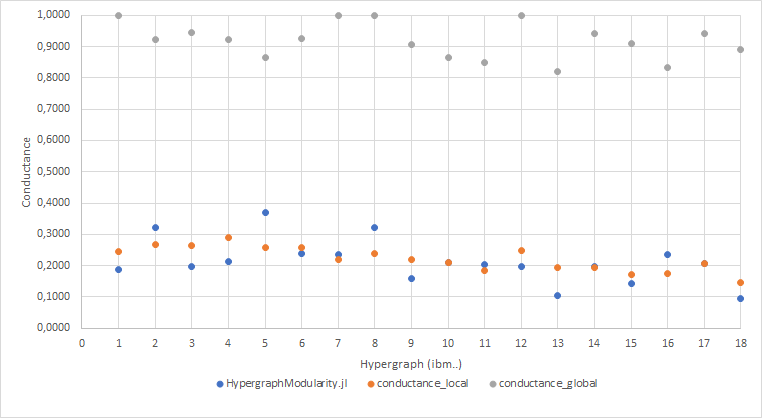
\includegraphics[width=0.6\textwidth]{conductance_comparison.png}
    \caption{Comparison of conductance of the partition.}
    \label{fig:conductance}
\end{figure}

To begin with, as \texttt{HyperModularity} decides the number of clusters $k$ 
automatically, we ran it first and then ran our algorithm with the same $k$ in 
different configurations. In the Table I~\ref{tab:comparison} we show the results 
of the comparison of \texttt{HyperModularity} against \textit{conductance\_local} 
and \textit{conductance\_global} with the random initial partitioner. We can see,
that \textit{conductance\_local} gives roughlt the same conductance as 
the \texttt{HyperModularity}, while \textit{conductance\_global} gives a much worse
result. Time-wise, both our implementations are much faster than 
\texttt{HyperModularity}.


\begin{figure}[t]
    \centering 
    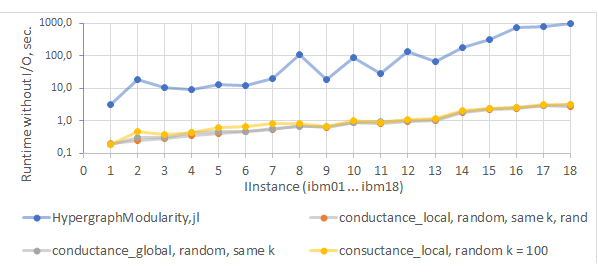
\includegraphics{time_comparison.png}
    \caption{Comparison of the run time against \texttt{HyperModularity}. The $y$-acsis is logarithmic}%
    \label{fig:time}
\end{figure}

To make the comparison more fair, we also ran \textit{conductance\_local} with the 
preset number of clusters $k = 100$ and the random initial partitioner. 
The results are shown in the Table~\ref{tab:comparison_k}. We can see, that
this way \textit{conductance\_local} gives a worse result than in the previous run,
but it is still close to the \texttt{HyperModularity}.

Figure~\ref{fig:conductance} and Figure~\ref{fig:time} summarize the conductance 
and the run time of this comparison. 

\medskip
Analogous experiments were run with the singleton initial partitioner, but the resulting
conductance of the clustering was always 1 except for rare 0.625 and 0.750. Therefore we 
don't include the results of these experiments in the report.

\subsection{Scalability of the algorithm}

\begin{table}
    \centering
    \begin{tabular}{|c|c|c|} \hline
        \textbf{Threads} & \textbf{Conductance} & \textbf{Run- and I/O-time} \\ \hline
        \textbf{1} & 0.5967 & 131.5407 s  + 3.4846 s \\ 
        \textbf{2} & 0.7283 & 74.2843 s + 2.1009 s \\ 
        \textbf{4} & 0.9369 & 46.9272 s  + 1.6002 s \\ 
        \textbf{8} & 0.6478 & 25.4402 s + 1.4921 s \\ 
        \textbf{16} & 0.7473 & 18.9490 s  + 1.5178 s \\ \hline
    \end{tabular}
    \caption{Performance of \textit{conductance\_local} with $k = 100$ 
    by increasing number of threads.}
    \label{tab:scalability_t}
\end{table}

The scalability of our implementation was tested only on the best configuration
(\textit{conductance\_local} with random initial partitioner) in two ways. First, 
we ran our algorithm on a large circuit-based hypergraph \texttt{circuit5M.mtx.hgr} 
with $5 558 326$ hyperedges and $59 524 291$ pins using 1, 2, 4, 8 and 16 threads.
The results are shown in the Table~\ref{tab:scalability_t}. We can see, that the 
running time of the algorithm decreases by about factor 2 with each next thread.
Unfortunately, the conductance of the clustering is not getting better with
the increase of the number of threads.

\smallskip
\noindent The second test was run on the same hypergraph, but with a different
number of clusters $k$. We ran the algorithm with $k = 100$, $k = 200$, $k = 400$, 
$k = 800$ and $k = 1600$. The results are shown in the Table~\ref{tab:scalability_k}. 
We can see, that the running time of the algorithm grows with the exponential increase 
of $k$, but not exponentially. Unfortunately, the conductance of the clustering is
getting worse and the number of clusters is not seemingly converging to some 
optimal number of "true" clusters. This is probably due to the fact, that with $k$
greater than the number of nodes in the coarsest hypergraph, random initial partitioner 
works similarily to singleton.

\begin{table}
    \centering
    \begin{tabular}{|c|c|c|c|} \hline
        \textbf{k} & \textbf{Conductance} & \textbf{Run- and I/O-time} & \textbf{\# clusters} \\ \hline
        \textbf{100} & 0.6483 & 42.3435 s + 5.1161 s & 100 \\ 
        \textbf{200} & 0.8326 & 50.0950 s + 1.6660 s & 198 \\ 
        \textbf{400} & 0.8597 & 46.2647 s + 1.6059 s & 376 \\ 
        \textbf{800} & 0.8272 & 61.7254 s + 5.12642 s & 623 \\ 
        \textbf{1600} & 0.9367 & 80.9240 s + 3.4388 s & 770 \\ \hline
    \end{tabular}
    \caption{The performance of \textit{conductance\_local} with random on 4 threads
    with increasing $k$}
    \label{tab:scalability_k}
\end{table}

\section{Conclusion}
\label{sec:conclusion}

The experimantal results show, that our implementation can find clustering
with conductance comparable to a state of the art hypergraph clustering and
needs significantly less time to do so, but the result heavily depends on 
the parameter $k$ and the initial partitioner.

\appendix
\section{Appendix}
\label{appendix:a}

\begin{theorem}
  Concuctance of a $k$-way partition $V_1, \dots, V_k$ is the maximal conductance 
  of a cut $V_i$ for $i = 1, \dots k$ with $V_i \neq \emptyset, V$. 
\end{theorem}
\begin{proof}
Without loss of generality, we can assume that the clusters $V_i$ are
non-empty (otherwise, we could remove the empty clusters from the 
partition whothout changing on eitther side of the equation discussed).
Per definition of conductance of a $k$-way partition, there exists a 
subset 
$\emptyset \subsetneq I \subsetneq \{1, \dots, k\}$ such that 
$\varphi(V_1, \dots V_k) = \varphi(\cup_{i \in I} V_i)$. Without loss 
of generality, we can further assume that the volume of the union of 
the clusters $V_i$ for $i \in I$ is less than or equal to the volume 
of its complement, \ie the volume of the union of all the clusters 
$V_i$ for $i \notin I$. Then we can write:
\begin{align*}
\varphi(V_1, \dots, V_k) 
&= 
\frac{\omega(\partial (\cup_{i \in I} V_i))}
     {\min(\vol(\cup_{i \in I} V_i), \vol(\cup_{i \notin I} V_i))} 
=
\frac{\sum \{\omega(e) : e - \text{a cutting edge of } \partial(\cup_{i \in I} V_i)\}}
     {\vol(\cup_{i \in I} V_i)}
\\ & \leq
\frac{\sum_{i \in I} \omega(\partial V_i)}
     {\sum_{i \in I} \vol(V_i)} 
=
\frac{\sum_{i \in I} \vol(V_i) \cdot \frac{\omega(\partial V_i)}
                                          {\vol(V_i)}}
     {\sum_{i \in I} \vol(V_i)} 
\leq
\max_{i \in I}\frac{\omega(\partial V_i)}
                   {\vol(V_i)}
\\ &\leq
\max_{i \in I}\frac{\omega(\partial V_i)}
                   {\min(\vol(V_i), \vol(V \backslash V_i))}
=
\max_{i \in I} \varphi(V_i)
\\ &\leq 
\varphi(V_1, \dots, V_k)
\end{align*}
Thus, all abothe written inequalities are equalities, which means that 
the conductance of the $k$-way partition is equal to the maximal 
conductance of a cut $V_i$ for $i = 1, \dots k$.

It is interesting to note that with this we have also proven that the 
conductance of a hypergraph partition is equal to the maximum ratio of 
the weight of a cut $V_i$ to the volume of the cluster $V_i$ over all 
the clusters $V_1, \dots V_k$. This property, however, was not used 
in the implementation due to late discovery.
\end{proof}


\bibliographystyle{plainnat}
\bibliography{references.bib}
\end{document}